\newpage
\section{Design pattern utilizzati}

\subsection{Introduzione}

\subsection{Abstract Factory}

\subsection{Publish - Subscribe}
Il Publish-Subscribe è un design pattern utilizzato per la comunicazione asincrona fra diversi processi, oggetti o altri agenti. I mittenti e i destinatari dialogano tramite data manager definiti come Broker o Dispatcher che svolgono la funzione di store-and-forward.
I mittenti (publisher) pubblicano i loro messaggi sui data manager e i destinatari (subscriber) si rivolgono al data manager abbonandosi (subscribing) alla ricezione del messaggio a cui sono interessati. Per garantire un sistema scalabile i publisher non sanno quanti e quali sono i subscriber e viceversa.
\begin{figure}[h]
	\centering
	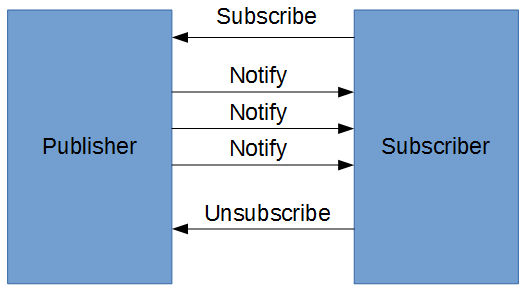
\includegraphics[width=0.5\linewidth]{IMG/pubsub}
	\caption{Design pattern Publish - Subscribe}
\end{figure}
I punti di forza di questo design pattern sono:
\begin{itemize}
	\item Totale disaccopiamento tra publisher e subscriber;
	\item Alta scalabilità nel software;
\end{itemize}

Nel progetto API Market il design pattern Publish-Subscribe sarà implementato come descritto sopra. Con l'utilizzo del framework MeteorJS la componente Broker o Dispatcher è completamente trasparente al programmatore, quindi è necessario pubblicare i dati e abbonarsi ad essi e MeteorJS si occuperà della comunicazione front-end/back-end.

\subsection{Singleton}